\documentclass[twoside]{article}

% Packages required by doxygen
\usepackage{fixltx2e}
\usepackage{calc}
\usepackage{doxygen}
\usepackage[export]{adjustbox} % also loads graphicx
\usepackage{graphicx}
\usepackage[utf8]{inputenc}
\usepackage{makeidx}
\usepackage{multicol}
\usepackage{multirow}
\PassOptionsToPackage{warn}{textcomp}
\usepackage{textcomp}
\usepackage[nointegrals]{wasysym}
\usepackage[table]{xcolor}

% NLS support packages
\usepackage{polski}
\usepackage[T1]{fontenc}

% Font selection
\usepackage[T1]{fontenc}
\usepackage[scaled=.90]{helvet}
\usepackage{courier}
\usepackage{amssymb}
\usepackage{sectsty}
\renewcommand{\familydefault}{\sfdefault}
\allsectionsfont{%
  \fontseries{bc}\selectfont%
  \color{darkgray}%
}
\renewcommand{\DoxyLabelFont}{%
  \fontseries{bc}\selectfont%
  \color{darkgray}%
}
\newcommand{\+}{\discretionary{\mbox{\scriptsize$\hookleftarrow$}}{}{}}

% Page & text layout
\usepackage{geometry}
\geometry{%
  a4paper,%
  top=2.5cm,%
  bottom=2.5cm,%
  left=2.5cm,%
  right=2.5cm%
}
\tolerance=750
\hfuzz=15pt
\hbadness=750
\setlength{\emergencystretch}{15pt}
\setlength{\parindent}{0cm}
\setlength{\parskip}{0.2cm}
\makeatletter
\renewcommand{\paragraph}{%
  \@startsection{paragraph}{4}{0ex}{-1.0ex}{1.0ex}{%
    \normalfont\normalsize\bfseries\SS@parafont%
  }%
}
\renewcommand{\subparagraph}{%
  \@startsection{subparagraph}{5}{0ex}{-1.0ex}{1.0ex}{%
    \normalfont\normalsize\bfseries\SS@subparafont%
  }%
}
\makeatother

% Headers & footers
\usepackage{fancyhdr}
\pagestyle{fancyplain}
\fancyhead[LE]{\fancyplain{}{\bfseries\thepage}}
\fancyhead[CE]{\fancyplain{}{}}
\fancyhead[RE]{\fancyplain{}{\bfseries\leftmark}}
\fancyhead[LO]{\fancyplain{}{\bfseries\rightmark}}
\fancyhead[CO]{\fancyplain{}{}}
\fancyhead[RO]{\fancyplain{}{\bfseries\thepage}}
\fancyfoot[LE]{\fancyplain{}{}}
\fancyfoot[CE]{\fancyplain{}{}}
\fancyfoot[RE]{\fancyplain{}{\bfseries\scriptsize Wygenerowano Śr, 27 maj 2015 13\+:06\+:26 dla Projektowanie algorytmów i metod sztucznej inteligencji. Laboratorium  9 -\/ Sprawozdanie programem Doxygen }}
\fancyfoot[LO]{\fancyplain{}{\bfseries\scriptsize Wygenerowano Śr, 27 maj 2015 13\+:06\+:26 dla Projektowanie algorytmów i metod sztucznej inteligencji. Laboratorium  9 -\/ Sprawozdanie programem Doxygen }}
\fancyfoot[CO]{\fancyplain{}{}}
\fancyfoot[RO]{\fancyplain{}{}}
\renewcommand{\footrulewidth}{0.4pt}
\renewcommand{\sectionmark}[1]{%
  \markright{\thesection\ #1}%
}

% Indices & bibliography
\usepackage{natbib}
\usepackage[titles]{tocloft}
\setcounter{tocdepth}{3}
\setcounter{secnumdepth}{5}
\makeindex

% Hyperlinks (required, but should be loaded last)
\usepackage{ifpdf}
\ifpdf
  \usepackage[pdftex,pagebackref=true]{hyperref}
\else
  \usepackage[ps2pdf,pagebackref=true]{hyperref}
\fi
\hypersetup{%
  colorlinks=true,%
  linkcolor=blue,%
  citecolor=blue,%
  unicode%
}

% Custom commands
\newcommand{\clearemptydoublepage}{%
  \newpage{\pagestyle{empty}\cleardoublepage}%
}


%===== C O N T E N T S =====

\begin{document}

% Titlepage & ToC
\hypersetup{pageanchor=false,
             bookmarks=true,
             bookmarksnumbered=true,
             pdfencoding=unicode
            }
\pagenumbering{roman}
\begin{titlepage}
\vspace*{7cm}
\begin{center}%
{\Large Projektowanie algorytmów i metod sztucznej inteligencji. Laboratorium 9 -\/ Sprawozdanie \\[1ex]\large 1.\+0 }\\
\vspace*{1cm}
{\large Wygenerowano przez Doxygen 1.8.9.1}\\
\vspace*{0.5cm}
{\small Śr, 27 maj 2015 13:06:26}\\
\end{center}
\end{titlepage}
\tableofcontents
\pagenumbering{arabic}
\hypersetup{pageanchor=true}

%--- Begin generated contents ---
\section{Projektowanie algorytm�w i metod sztucznej inteligencji. Laboratorium 9 -\/ Sprawozdanie}
\label{index}\hypertarget{index}{}\begin{DoxyAuthor}{Autor}
Wojciech Makuch 
\end{DoxyAuthor}
\begin{DoxyDate}{Data}
27.\+05.\+2015 
\end{DoxyDate}
\begin{DoxyVersion}{Wersja}
1.\+0
\end{DoxyVersion}
program testujacy oraz benchmarkujacy zaimplementowane grafy posiada menu uzytkownika do wyboru \hypertarget{index_utworz}{}\subsection{graf}\label{index_utworz}
\hypertarget{index_utworz}{}\subsection{graf}\label{index_utworz}
\hypertarget{index_wyswietl}{}\subsection{macierz sasiedztwa}\label{index_wyswietl}
\hypertarget{index_DSF}{}\subsection{D\+S\+F}\label{index_DSF}
\hypertarget{index_BFS}{}\subsection{B\+F\+S}\label{index_BFS}
\hypertarget{index_benchmarkuj}{}\subsection{D\+F\+Sa}\label{index_benchmarkuj}
\hypertarget{index_benchmarkuj}{}\subsection{D\+F\+Sa}\label{index_benchmarkuj}
\hypertarget{index_graf}{}\subsection{omawiany na cwiczeniach}\label{index_graf}
\hypertarget{main.cpp_wyjscie}{}\subsection{wyjscie}\label{main.cpp_wyjscie}

\section{Indeks hierarchiczny}
\subsection{Class Hierarchy}
This inheritance list is sorted roughly, but not completely, alphabetically\+:\begin{DoxyCompactList}
\item \contentsline{section}{C\+Benchmark}{\pageref{class_c_benchmark}}{}
\begin{DoxyCompactList}
\item \contentsline{section}{C\+Sort}{\pageref{class_c_sort}}{}
\begin{DoxyCompactList}
\item \contentsline{section}{C\+Heap\+Sort}{\pageref{class_c_heap_sort}}{}
\item \contentsline{section}{C\+Merge\+Sort}{\pageref{class_c_merge_sort}}{}
\item \contentsline{section}{C\+Quick\+Sort}{\pageref{class_c_quick_sort}}{}
\end{DoxyCompactList}
\end{DoxyCompactList}
\item \contentsline{section}{C\+List}{\pageref{class_c_list}}{}
\end{DoxyCompactList}

\section{Indeks klas}
\subsection{Lista klas}
Tutaj znajdują się klasy, struktury, unie i interfejsy wraz z ich krótkimi opisami\+:\begin{DoxyCompactList}
\item\contentsline{section}{\hyperlink{class_c_benchmark}{C\+Benchmark} }{\pageref{class_c_benchmark}}{}
\item\contentsline{section}{\hyperlink{class_c_edge}{C\+Edge} \\*Definicja klasy \hyperlink{class_c_edge}{C\+Edge} definuje krawedz grafu nie zawiera wag }{\pageref{class_c_edge}}{}
\item\contentsline{section}{\hyperlink{class_c_graph}{C\+Graph} \\*Definicja klasy \hyperlink{class_c_graph}{C\+Graph} definije graf skierowany bez wagowaych krawedzi dziedzicy po klasie \hyperlink{class_c_benchmark}{C\+Benchmark} }{\pageref{class_c_graph}}{}
\item\contentsline{section}{\hyperlink{class_c_node}{C\+Node} \\*Definicja klasy \hyperlink{class_c_node}{C\+Node} definiuje pojedynczy wezel grafu }{\pageref{class_c_node}}{}
\item\contentsline{section}{\hyperlink{classqueue}{queue} \\*Definicja klasy queue definicja kolejki A\+D\+T, kolejka typu F\+I\+F\+O zimplementowaa na liscie }{\pageref{classqueue}}{}
\item\contentsline{section}{\hyperlink{classqueue__node}{queue\+\_\+node} \\*Definicja klasy \hyperlink{classqueue__node}{queue\+\_\+node} definicja wezla dla kolejki definiuje pojedynczy element bedacy w kolejkce }{\pageref{classqueue__node}}{}
\end{DoxyCompactList}

\section{Indeks plików}
\subsection{Lista plików}
Tutaj znajduje się lista wszystkich plików z ich krótkimi opisami\+:\begin{DoxyCompactList}
\item\contentsline{section}{\hyperlink{format_8h}{format.\+h} }{\pageref{format_8h}}{}
\item\contentsline{section}{\hyperlink{global_8h}{global.\+h} }{\pageref{global_8h}}{}
\item\contentsline{section}{\hyperlink{graph_8cpp}{graph.\+cpp} \\*Implementuje zdefiniowana klase grafu }{\pageref{graph_8cpp}}{}
\item\contentsline{section}{\hyperlink{graph_8hh}{graph.\+hh} \\*Zwiera definicje klas \hyperlink{class_c_node}{C\+Node}, \hyperlink{class_c_edge}{C\+Edge}, C\+Grpah \hyperlink{class_c_node}{C\+Node} -\/ wezel grafu \hyperlink{class_c_edge}{C\+Edge} -\/ krawedz grafu \hyperlink{class_c_graph}{C\+Graph} -\/ graf }{\pageref{graph_8hh}}{}
\item\contentsline{section}{\hyperlink{main_8cpp}{main.\+cpp} }{\pageref{main_8cpp}}{}
\item\contentsline{section}{\hyperlink{queue_8cpp}{queue.\+cpp} \\*Implementuje zdefiniowana klase kolejki }{\pageref{queue_8cpp}}{}
\item\contentsline{section}{\hyperlink{queue_8hh}{queue.\+hh} \\*Zawiera definicje klas \hyperlink{classqueue__node}{queue\+\_\+node}, queue \hyperlink{classqueue__node}{queue\+\_\+node} -\/ wezel kolejki queue -\/ kolejka }{\pageref{queue_8hh}}{}
\item\contentsline{section}{\hyperlink{stack_8hh}{stack.\+hh} \\*Definicja struktury danych \hyperlink{class_lista}{Lista} }{\pageref{stack_8hh}}{}
\end{DoxyCompactList}

\section{Dokumentacja klas}
\hypertarget{class_c_benchmark}{}\subsection{Dokumentacja klasy C\+Benchmark}
\label{class_c_benchmark}\index{C\+Benchmark@{C\+Benchmark}}


{\ttfamily \#include $<$benchmark.\+hh$>$}



Dziedziczona przez \hyperlink{class_c_graph}{C\+Graph}.

\subsubsection*{Metody publiczne}
\begin{DoxyCompactItemize}
\item 
virtual void \hyperlink{class_c_benchmark_aa6f22bf0b316b51db8f439c7420a1666}{start\+\_\+timer} ()
\begin{DoxyCompactList}\small\item\em definicja metody start\+\_\+timer rozpoczyna pomiar czasu zapisuje dane do zmiennej performance\+Count\+Start korzysta z metdoy Start\+Timer() \end{DoxyCompactList}\item 
virtual void \hyperlink{class_c_benchmark_a945aaa453776cd11395166b470d11778}{stop\+\_\+timer} ()
\begin{DoxyCompactList}\small\item\em definicja metody stop\+\_\+timer konczy pomiar czasu zapsiuje dane do zmiennej performance\+Count\+End korzysta z metody end\+Timer \end{DoxyCompactList}\item 
virtual int \hyperlink{class_c_benchmark_acb3046f4f9fdff7c17c7633baf41cf36}{put\+\_\+time\+\_\+to\+\_\+file} (int size\+\_\+of\+\_\+list)
\begin{DoxyCompactList}\small\item\em definicja metody put\+\_\+time\+\_\+to\+\_\+file otiwra plik o nazwie \textquotesingle{}timing.\+txt\textquotesingle{} zapisuje do niego ilosc elementow listy oraz czas przeprowadzenia operacji przez klasy obserwowane zamyka plik. \end{DoxyCompactList}\end{DoxyCompactItemize}
\subsubsection*{Metody prywatne}
\begin{DoxyCompactItemize}
\item 
L\+A\+R\+G\+E\+\_\+\+I\+N\+T\+E\+G\+E\+R \hyperlink{class_c_benchmark_a43dd8d9d01499e28f1dc899ea6f3ed97}{start\+Timer} ()
\item 
L\+A\+R\+G\+E\+\_\+\+I\+N\+T\+E\+G\+E\+R \hyperlink{class_c_benchmark_aab174262b346c522bdbc1df87ed93532}{end\+Timer} ()
\end{DoxyCompactItemize}
\subsubsection*{Atrybuty prywatne}
\begin{DoxyCompactItemize}
\item 
L\+A\+R\+G\+E\+\_\+\+I\+N\+T\+E\+G\+E\+R \hyperlink{class_c_benchmark_a54ec1bb4f1e570341e14adfc6312f1b7}{performance\+Count\+Start}
\item 
L\+A\+R\+G\+E\+\_\+\+I\+N\+T\+E\+G\+E\+R \hyperlink{class_c_benchmark_ae72cb7dad8bf32730109776d546af2ad}{performance\+Count\+End}
\end{DoxyCompactItemize}


\subsubsection{Opis szczegółowy}
definicja klasy \hyperlink{class_c_benchmark}{C\+Benchmark} definijue stoper zliczajacy czas wykoania operacji przez inne klasy jest przykladem wzorca obserwatora obserwuje klase C\+Sort i zlicza czas sortowania listy 

Definicja w linii 16 pliku benchmark.\+hh.



\subsubsection{Dokumentacja funkcji składowych}
\hypertarget{class_c_benchmark_aab174262b346c522bdbc1df87ed93532}{}\index{C\+Benchmark@{C\+Benchmark}!end\+Timer@{end\+Timer}}
\index{end\+Timer@{end\+Timer}!C\+Benchmark@{C\+Benchmark}}
\paragraph[{end\+Timer}]{\setlength{\rightskip}{0pt plus 5cm}L\+A\+R\+G\+E\+\_\+\+I\+N\+T\+E\+G\+E\+R C\+Benchmark\+::end\+Timer (
\begin{DoxyParamCaption}
{}
\end{DoxyParamCaption}
)\hspace{0.3cm}{\ttfamily [private]}}\label{class_c_benchmark_aab174262b346c522bdbc1df87ed93532}


Definicja w linii 19 pliku benchmark.\+cpp.

\hypertarget{class_c_benchmark_acb3046f4f9fdff7c17c7633baf41cf36}{}\index{C\+Benchmark@{C\+Benchmark}!put\+\_\+time\+\_\+to\+\_\+file@{put\+\_\+time\+\_\+to\+\_\+file}}
\index{put\+\_\+time\+\_\+to\+\_\+file@{put\+\_\+time\+\_\+to\+\_\+file}!C\+Benchmark@{C\+Benchmark}}
\paragraph[{put\+\_\+time\+\_\+to\+\_\+file}]{\setlength{\rightskip}{0pt plus 5cm}int C\+Benchmark\+::put\+\_\+time\+\_\+to\+\_\+file (
\begin{DoxyParamCaption}
\item[{int}]{size\+\_\+of\+\_\+list}
\end{DoxyParamCaption}
)\hspace{0.3cm}{\ttfamily [virtual]}}\label{class_c_benchmark_acb3046f4f9fdff7c17c7633baf41cf36}

\begin{DoxyParams}{Parametry}
{\em size\+\_\+of\+\_\+list} & -\/ rozmiar listy \\
\hline
\end{DoxyParams}
\begin{DoxyReturn}{Zwraca}
czas przeprowadzenia operacji 

-\/1 w przypadu bledu otwarcia pliku 
\end{DoxyReturn}


Definicja w linii 38 pliku benchmark.\+cpp.

\hypertarget{class_c_benchmark_aa6f22bf0b316b51db8f439c7420a1666}{}\index{C\+Benchmark@{C\+Benchmark}!start\+\_\+timer@{start\+\_\+timer}}
\index{start\+\_\+timer@{start\+\_\+timer}!C\+Benchmark@{C\+Benchmark}}
\paragraph[{start\+\_\+timer}]{\setlength{\rightskip}{0pt plus 5cm}void C\+Benchmark\+::start\+\_\+timer (
\begin{DoxyParamCaption}
{}
\end{DoxyParamCaption}
)\hspace{0.3cm}{\ttfamily [virtual]}}\label{class_c_benchmark_aa6f22bf0b316b51db8f439c7420a1666}


Definicja w linii 28 pliku benchmark.\+cpp.

\hypertarget{class_c_benchmark_a43dd8d9d01499e28f1dc899ea6f3ed97}{}\index{C\+Benchmark@{C\+Benchmark}!start\+Timer@{start\+Timer}}
\index{start\+Timer@{start\+Timer}!C\+Benchmark@{C\+Benchmark}}
\paragraph[{start\+Timer}]{\setlength{\rightskip}{0pt plus 5cm}L\+A\+R\+G\+E\+\_\+\+I\+N\+T\+E\+G\+E\+R C\+Benchmark\+::start\+Timer (
\begin{DoxyParamCaption}
{}
\end{DoxyParamCaption}
)\hspace{0.3cm}{\ttfamily [private]}}\label{class_c_benchmark_a43dd8d9d01499e28f1dc899ea6f3ed97}


Definicja w linii 10 pliku benchmark.\+cpp.

\hypertarget{class_c_benchmark_a945aaa453776cd11395166b470d11778}{}\index{C\+Benchmark@{C\+Benchmark}!stop\+\_\+timer@{stop\+\_\+timer}}
\index{stop\+\_\+timer@{stop\+\_\+timer}!C\+Benchmark@{C\+Benchmark}}
\paragraph[{stop\+\_\+timer}]{\setlength{\rightskip}{0pt plus 5cm}void C\+Benchmark\+::stop\+\_\+timer (
\begin{DoxyParamCaption}
{}
\end{DoxyParamCaption}
)\hspace{0.3cm}{\ttfamily [virtual]}}\label{class_c_benchmark_a945aaa453776cd11395166b470d11778}


Definicja w linii 33 pliku benchmark.\+cpp.



\subsubsection{Dokumentacja atrybutów składowych}
\hypertarget{class_c_benchmark_ae72cb7dad8bf32730109776d546af2ad}{}\index{C\+Benchmark@{C\+Benchmark}!performance\+Count\+End@{performance\+Count\+End}}
\index{performance\+Count\+End@{performance\+Count\+End}!C\+Benchmark@{C\+Benchmark}}
\paragraph[{performance\+Count\+End}]{\setlength{\rightskip}{0pt plus 5cm}L\+A\+R\+G\+E\+\_\+\+I\+N\+T\+E\+G\+E\+R C\+Benchmark\+::performance\+Count\+End\hspace{0.3cm}{\ttfamily [private]}}\label{class_c_benchmark_ae72cb7dad8bf32730109776d546af2ad}


Definicja w linii 18 pliku benchmark.\+hh.

\hypertarget{class_c_benchmark_a54ec1bb4f1e570341e14adfc6312f1b7}{}\index{C\+Benchmark@{C\+Benchmark}!performance\+Count\+Start@{performance\+Count\+Start}}
\index{performance\+Count\+Start@{performance\+Count\+Start}!C\+Benchmark@{C\+Benchmark}}
\paragraph[{performance\+Count\+Start}]{\setlength{\rightskip}{0pt plus 5cm}L\+A\+R\+G\+E\+\_\+\+I\+N\+T\+E\+G\+E\+R C\+Benchmark\+::performance\+Count\+Start\hspace{0.3cm}{\ttfamily [private]}}\label{class_c_benchmark_a54ec1bb4f1e570341e14adfc6312f1b7}


Definicja w linii 17 pliku benchmark.\+hh.



Dokumentacja dla tej klasy została wygenerowana z plików\+:\begin{DoxyCompactItemize}
\item 
\hyperlink{benchmark_8hh}{benchmark.\+hh}\item 
\hyperlink{benchmark_8cpp}{benchmark.\+cpp}\end{DoxyCompactItemize}

\hypertarget{class_c_edge}{}\subsection{Dokumentacja klasy C\+Edge}
\label{class_c_edge}\index{C\+Edge@{C\+Edge}}


definicja klasy \hyperlink{class_c_edge}{C\+Edge} definuje krawedz grafu nie zawiera wag  




{\ttfamily \#include $<$graph.\+hh$>$}

\subsubsection*{Atrybuty prywatne}
\begin{DoxyCompactItemize}
\item 
\hyperlink{class_c_node}{C\+Node} $\ast$ \hyperlink{class_c_edge_a6028b71c45755a0f37cd6e240b357bac}{prev}
\item 
\hyperlink{class_c_node}{C\+Node} $\ast$ \hyperlink{class_c_edge_ad1ee614fba28429ff44c5c793676cbd4}{next}
\end{DoxyCompactItemize}
\subsubsection*{Przyjaciele}
\begin{DoxyCompactItemize}
\item 
class \hyperlink{class_c_edge_a5ba04087b017dfeadb708ba91d6daf1b}{C\+Graph}
\end{DoxyCompactItemize}


\subsubsection{Opis szczegółowy}


Definicja w linii 29 pliku graph.\+hh.



\subsubsection{Dokumentacja przyjaciół i funkcji związanych}
\hypertarget{class_c_edge_a5ba04087b017dfeadb708ba91d6daf1b}{}\index{C\+Edge@{C\+Edge}!C\+Graph@{C\+Graph}}
\index{C\+Graph@{C\+Graph}!C\+Edge@{C\+Edge}}
\paragraph[{C\+Graph}]{\setlength{\rightskip}{0pt plus 5cm}friend class {\bf C\+Graph}\hspace{0.3cm}{\ttfamily [friend]}}\label{class_c_edge_a5ba04087b017dfeadb708ba91d6daf1b}


Definicja w linii 30 pliku graph.\+hh.



\subsubsection{Dokumentacja atrybutów składowych}
\hypertarget{class_c_edge_ad1ee614fba28429ff44c5c793676cbd4}{}\index{C\+Edge@{C\+Edge}!next@{next}}
\index{next@{next}!C\+Edge@{C\+Edge}}
\paragraph[{next}]{\setlength{\rightskip}{0pt plus 5cm}{\bf C\+Node}$\ast$ C\+Edge\+::next\hspace{0.3cm}{\ttfamily [private]}}\label{class_c_edge_ad1ee614fba28429ff44c5c793676cbd4}
wskaznik na poprzedni wezel 

Definicja w linii 32 pliku graph.\+hh.

\hypertarget{class_c_edge_a6028b71c45755a0f37cd6e240b357bac}{}\index{C\+Edge@{C\+Edge}!prev@{prev}}
\index{prev@{prev}!C\+Edge@{C\+Edge}}
\paragraph[{prev}]{\setlength{\rightskip}{0pt plus 5cm}{\bf C\+Node}$\ast$ C\+Edge\+::prev\hspace{0.3cm}{\ttfamily [private]}}\label{class_c_edge_a6028b71c45755a0f37cd6e240b357bac}


Definicja w linii 31 pliku graph.\+hh.



Dokumentacja dla tej klasy została wygenerowana z pliku\+:\begin{DoxyCompactItemize}
\item 
\hyperlink{graph_8hh}{graph.\+hh}\end{DoxyCompactItemize}

\hypertarget{class_c_graph}{}\subsection{Dokumentacja klasy C\+Graph}
\label{class_c_graph}\index{C\+Graph@{C\+Graph}}


definicja klasy \hyperlink{class_c_graph}{C\+Graph} definije graf skierowany bez wagowaych krawedzi dziedzicy po klasie C\+Benchmark  




{\ttfamily \#include $<$graph.\+hh$>$}

\subsubsection*{Metody publiczne}
\begin{DoxyCompactItemize}
\item 
\hyperlink{class_c_graph_a6568f9df5401061719c6b31111092df2}{C\+Graph} (int v, int e)
\begin{DoxyCompactList}\small\item\em definicja konstruktora parametrycznego alokuje pamiec dla tablic wezlow krawdzi oraz dla macierzy sasiedztwa \end{DoxyCompactList}\item 
\hyperlink{class_c_graph_af939e78d0fef6cea7711ae44f58f5a16}{$\sim$\+C\+Graph} ()
\begin{DoxyCompactList}\small\item\em definicja destruktora \end{DoxyCompactList}\item 
void \hyperlink{class_c_graph_ab400ede6f6abdb683b4f099df1f05edd}{set\+\_\+graph} (int vertice1, int vertice2)
\begin{DoxyCompactList}\small\item\em definicja metody set\+\_\+graph wiaze wezly wskaznikami krawdziom ustawia odpowiednie wezly wypelnia macierz sasiedztwa \end{DoxyCompactList}\item 
void \hyperlink{class_c_graph_a173a387b56acf5035e120f7ec4d144ae}{print\+\_\+matrix} () const 
\begin{DoxyCompactList}\small\item\em definicja metody print\+\_\+maatrix wyswietla macierz sasiedztwa \end{DoxyCompactList}\item 
void \hyperlink{class_c_graph_a995e1f160b774b1d0c73dc1e3d6df5a4}{D\+F\+S} (int v)
\begin{DoxyCompactList}\small\item\em definicja metody D\+F\+Sing przeszukuje graf algorytmem D\+F\+S (przeszukiwanie w glab) zaimplementowana rekuencyjnie wykorzystana w metodzie D\+F\+S wyposarzonej w timery \end{DoxyCompactList}\item 
void \hyperlink{class_c_graph_a7959dedbebc0e036672eae63e25e96eb}{B\+F\+S} (int v)
\begin{DoxyCompactList}\small\item\em definicja metody D\+F\+S wywoluje metode D\+F\+Sing posiada timery zapisujace zmierzony czas do pliku \end{DoxyCompactList}\item 
void \hyperlink{class_c_graph_a3af9d81bcc5baf54d713a78713d164de}{save\+\_\+matrix} (std\+::fstream \&file) const 
\begin{DoxyCompactList}\small\item\em definicja metody save\+\_\+matrix zapsiuje macierz saciedztwa do pliku \end{DoxyCompactList}\item 
bool \hyperlink{class_c_graph_a34997383af6ab4eb69372f7f1259f2e8}{B\+F\+S\+Path} (int start, int meta, \hyperlink{class_lista}{Lista}$<$ int $>$ $\ast$L)
\begin{DoxyCompactList}\small\item\em definicja metody B\+F\+S\+Path Oblicza najszybsza sciezke w grafie miedzy punktem startowym, a koncowym i zapisuje ja na stosie \end{DoxyCompactList}\end{DoxyCompactItemize}
\subsubsection*{Atrybuty publiczne}
\begin{DoxyCompactItemize}
\item 
int \hyperlink{class_c_graph_a76914f22c12c93e293c392342a4a233c}{V}
\item 
int \hyperlink{class_c_graph_a2bd3b0ae57901636d327bc7a6fdab545}{E}
\item 
int $\ast$$\ast$ \hyperlink{class_c_graph_a53c8f8a69d4d041b8b7557b5fece2f58}{matrix}
\item 
bool $\ast$ \hyperlink{class_c_graph_a8478f38bd0487246450f933dc4403227}{visited}
\end{DoxyCompactItemize}


\subsubsection{Opis szczegółowy}


Definicja w linii 42 pliku graph.\+hh.



\subsubsection{Dokumentacja konstruktora i destruktora}
\hypertarget{class_c_graph_a6568f9df5401061719c6b31111092df2}{}\index{C\+Graph@{C\+Graph}!C\+Graph@{C\+Graph}}
\index{C\+Graph@{C\+Graph}!C\+Graph@{C\+Graph}}
\paragraph[{C\+Graph}]{\setlength{\rightskip}{0pt plus 5cm}C\+Graph\+::\+C\+Graph (
\begin{DoxyParamCaption}
\item[{int}]{v, }
\item[{int}]{e}
\end{DoxyParamCaption}
)}\label{class_c_graph_a6568f9df5401061719c6b31111092df2}
lista odwiedzonych elementow grafu


\begin{DoxyParams}{Parametry}
{\em v} & ilosc wezlow \\
\hline
{\em e} & ilosc krawedzi \\
\hline
\end{DoxyParams}


Definicja w linii 25 pliku graph.\+cpp.

\hypertarget{class_c_graph_af939e78d0fef6cea7711ae44f58f5a16}{}\index{C\+Graph@{C\+Graph}!````~C\+Graph@{$\sim$\+C\+Graph}}
\index{````~C\+Graph@{$\sim$\+C\+Graph}!C\+Graph@{C\+Graph}}
\paragraph[{$\sim$\+C\+Graph}]{\setlength{\rightskip}{0pt plus 5cm}C\+Graph\+::$\sim$\+C\+Graph (
\begin{DoxyParamCaption}
{}
\end{DoxyParamCaption}
)}\label{class_c_graph_af939e78d0fef6cea7711ae44f58f5a16}


Definicja w linii 41 pliku graph.\+cpp.



\subsubsection{Dokumentacja funkcji składowych}
\hypertarget{class_c_graph_a7959dedbebc0e036672eae63e25e96eb}{}\index{C\+Graph@{C\+Graph}!B\+F\+S@{B\+F\+S}}
\index{B\+F\+S@{B\+F\+S}!C\+Graph@{C\+Graph}}
\paragraph[{B\+F\+S}]{\setlength{\rightskip}{0pt plus 5cm}void C\+Graph\+::\+B\+F\+S (
\begin{DoxyParamCaption}
\item[{int}]{v}
\end{DoxyParamCaption}
)}\label{class_c_graph_a7959dedbebc0e036672eae63e25e96eb}

\begin{DoxyParams}{Parametry}
{\em v} & element poczatkowy od ktorego algorytm D\+F\+S rozpoczyna przeszukiwanie \\
\hline
\end{DoxyParams}


Definicja w linii 80 pliku graph.\+cpp.

\hypertarget{class_c_graph_a34997383af6ab4eb69372f7f1259f2e8}{}\index{C\+Graph@{C\+Graph}!B\+F\+S\+Path@{B\+F\+S\+Path}}
\index{B\+F\+S\+Path@{B\+F\+S\+Path}!C\+Graph@{C\+Graph}}
\paragraph[{B\+F\+S\+Path}]{\setlength{\rightskip}{0pt plus 5cm}bool C\+Graph\+::\+B\+F\+S\+Path (
\begin{DoxyParamCaption}
\item[{int}]{start, }
\item[{int}]{meta, }
\item[{{\bf Lista}$<$ int $>$ $\ast$}]{L}
\end{DoxyParamCaption}
)}\label{class_c_graph_a34997383af6ab4eb69372f7f1259f2e8}

\begin{DoxyParams}{Parametry}
{\em start} & punkt startowy \\
\hline
{\em meta} & punkt koncowy \\
\hline
{\em $\ast$\+L} & wskaznik do stosu, na ktorym sa zapisane elementy \\
\hline
\end{DoxyParams}


Definicja w linii 109 pliku graph.\+cpp.

\hypertarget{class_c_graph_a995e1f160b774b1d0c73dc1e3d6df5a4}{}\index{C\+Graph@{C\+Graph}!D\+F\+S@{D\+F\+S}}
\index{D\+F\+S@{D\+F\+S}!C\+Graph@{C\+Graph}}
\paragraph[{D\+F\+S}]{\setlength{\rightskip}{0pt plus 5cm}void C\+Graph\+::\+D\+F\+S (
\begin{DoxyParamCaption}
\item[{int}]{v}
\end{DoxyParamCaption}
)}\label{class_c_graph_a995e1f160b774b1d0c73dc1e3d6df5a4}

\begin{DoxyParams}{Parametry}
{\em v} & element poczatkowy od ktorego algorytm rozpoczyna przeszukiwanie \\
\hline
\end{DoxyParams}


Definicja w linii 68 pliku graph.\+cpp.

\hypertarget{class_c_graph_a173a387b56acf5035e120f7ec4d144ae}{}\index{C\+Graph@{C\+Graph}!print\+\_\+matrix@{print\+\_\+matrix}}
\index{print\+\_\+matrix@{print\+\_\+matrix}!C\+Graph@{C\+Graph}}
\paragraph[{print\+\_\+matrix}]{\setlength{\rightskip}{0pt plus 5cm}void C\+Graph\+::print\+\_\+matrix (
\begin{DoxyParamCaption}
{}
\end{DoxyParamCaption}
) const}\label{class_c_graph_a173a387b56acf5035e120f7ec4d144ae}


Definicja w linii 58 pliku graph.\+cpp.

\hypertarget{class_c_graph_a3af9d81bcc5baf54d713a78713d164de}{}\index{C\+Graph@{C\+Graph}!save\+\_\+matrix@{save\+\_\+matrix}}
\index{save\+\_\+matrix@{save\+\_\+matrix}!C\+Graph@{C\+Graph}}
\paragraph[{save\+\_\+matrix}]{\setlength{\rightskip}{0pt plus 5cm}void C\+Graph\+::save\+\_\+matrix (
\begin{DoxyParamCaption}
\item[{std\+::fstream \&}]{file}
\end{DoxyParamCaption}
) const}\label{class_c_graph_a3af9d81bcc5baf54d713a78713d164de}

\begin{DoxyParams}{Parametry}
{\em file} & uchwyt do pliku \\
\hline
\end{DoxyParams}


Definicja w linii 15 pliku graph.\+cpp.

\hypertarget{class_c_graph_ab400ede6f6abdb683b4f099df1f05edd}{}\index{C\+Graph@{C\+Graph}!set\+\_\+graph@{set\+\_\+graph}}
\index{set\+\_\+graph@{set\+\_\+graph}!C\+Graph@{C\+Graph}}
\paragraph[{set\+\_\+graph}]{\setlength{\rightskip}{0pt plus 5cm}void C\+Graph\+::set\+\_\+graph (
\begin{DoxyParamCaption}
\item[{int}]{vertice1, }
\item[{int}]{vertice2}
\end{DoxyParamCaption}
)}\label{class_c_graph_ab400ede6f6abdb683b4f099df1f05edd}

\begin{DoxyParams}{Parametry}
{\em edge1} & krawdz do ktorej przypisujemy poszczegolne wierzcholki \\
\hline
{\em vertice1} & przypisywany pierwszy wierzcholek \\
\hline
{\em vertice2} & przypisywany drugi wierzcholek \\
\hline
\end{DoxyParams}


Definicja w linii 52 pliku graph.\+cpp.



\subsubsection{Dokumentacja atrybutów składowych}
\hypertarget{class_c_graph_a2bd3b0ae57901636d327bc7a6fdab545}{}\index{C\+Graph@{C\+Graph}!E@{E}}
\index{E@{E}!C\+Graph@{C\+Graph}}
\paragraph[{E}]{\setlength{\rightskip}{0pt plus 5cm}int C\+Graph\+::\+E}\label{class_c_graph_a2bd3b0ae57901636d327bc7a6fdab545}
ilosc wezlow 

Definicja w linii 45 pliku graph.\+hh.

\hypertarget{class_c_graph_a53c8f8a69d4d041b8b7557b5fece2f58}{}\index{C\+Graph@{C\+Graph}!matrix@{matrix}}
\index{matrix@{matrix}!C\+Graph@{C\+Graph}}
\paragraph[{matrix}]{\setlength{\rightskip}{0pt plus 5cm}int$\ast$$\ast$ C\+Graph\+::matrix}\label{class_c_graph_a53c8f8a69d4d041b8b7557b5fece2f58}
ilosc krawedzi 

Definicja w linii 47 pliku graph.\+hh.

\hypertarget{class_c_graph_a76914f22c12c93e293c392342a4a233c}{}\index{C\+Graph@{C\+Graph}!V@{V}}
\index{V@{V}!C\+Graph@{C\+Graph}}
\paragraph[{V}]{\setlength{\rightskip}{0pt plus 5cm}int C\+Graph\+::\+V}\label{class_c_graph_a76914f22c12c93e293c392342a4a233c}


Definicja w linii 44 pliku graph.\+hh.

\hypertarget{class_c_graph_a8478f38bd0487246450f933dc4403227}{}\index{C\+Graph@{C\+Graph}!visited@{visited}}
\index{visited@{visited}!C\+Graph@{C\+Graph}}
\paragraph[{visited}]{\setlength{\rightskip}{0pt plus 5cm}bool$\ast$ C\+Graph\+::visited}\label{class_c_graph_a8478f38bd0487246450f933dc4403227}
macierz sasiedztwa 

Definicja w linii 48 pliku graph.\+hh.



Dokumentacja dla tej klasy została wygenerowana z plików\+:\begin{DoxyCompactItemize}
\item 
\hyperlink{graph_8hh}{graph.\+hh}\item 
\hyperlink{graph_8cpp}{graph.\+cpp}\end{DoxyCompactItemize}

\hypertarget{class_c_node}{}\subsection{Dokumentacja klasy C\+Node}
\label{class_c_node}\index{C\+Node@{C\+Node}}


definicja klasy \hyperlink{class_c_node}{C\+Node} definiuje pojedynczy wezel grafu  




{\ttfamily \#include $<$graph.\+hh$>$}

\subsubsection*{Atrybuty prywatne}
\begin{DoxyCompactItemize}
\item 
int \hyperlink{class_c_node_ad08aa99402f6cfbbb9d9580d1f001441}{value}
\end{DoxyCompactItemize}
\subsubsection*{Przyjaciele}
\begin{DoxyCompactItemize}
\item 
class \hyperlink{class_c_node_a0447ad471d74d1dfa4bfd184bccd1b36}{C\+Edge}
\item 
class \hyperlink{class_c_node_a5ba04087b017dfeadb708ba91d6daf1b}{C\+Graph}
\end{DoxyCompactItemize}


\subsubsection{Opis szczegółowy}


Definicja w linii 18 pliku graph.\+hh.



\subsubsection{Dokumentacja przyjaciół i funkcji związanych}
\hypertarget{class_c_node_a0447ad471d74d1dfa4bfd184bccd1b36}{}\index{C\+Node@{C\+Node}!C\+Edge@{C\+Edge}}
\index{C\+Edge@{C\+Edge}!C\+Node@{C\+Node}}
\paragraph[{C\+Edge}]{\setlength{\rightskip}{0pt plus 5cm}friend class {\bf C\+Edge}\hspace{0.3cm}{\ttfamily [friend]}}\label{class_c_node_a0447ad471d74d1dfa4bfd184bccd1b36}


Definicja w linii 19 pliku graph.\+hh.

\hypertarget{class_c_node_a5ba04087b017dfeadb708ba91d6daf1b}{}\index{C\+Node@{C\+Node}!C\+Graph@{C\+Graph}}
\index{C\+Graph@{C\+Graph}!C\+Node@{C\+Node}}
\paragraph[{C\+Graph}]{\setlength{\rightskip}{0pt plus 5cm}friend class {\bf C\+Graph}\hspace{0.3cm}{\ttfamily [friend]}}\label{class_c_node_a5ba04087b017dfeadb708ba91d6daf1b}


Definicja w linii 20 pliku graph.\+hh.



\subsubsection{Dokumentacja atrybutów składowych}
\hypertarget{class_c_node_ad08aa99402f6cfbbb9d9580d1f001441}{}\index{C\+Node@{C\+Node}!value@{value}}
\index{value@{value}!C\+Node@{C\+Node}}
\paragraph[{value}]{\setlength{\rightskip}{0pt plus 5cm}int C\+Node\+::value\hspace{0.3cm}{\ttfamily [private]}}\label{class_c_node_ad08aa99402f6cfbbb9d9580d1f001441}


Definicja w linii 21 pliku graph.\+hh.



Dokumentacja dla tej klasy została wygenerowana z pliku\+:\begin{DoxyCompactItemize}
\item 
\hyperlink{graph_8hh}{graph.\+hh}\end{DoxyCompactItemize}

\hypertarget{classqueue}{}\subsection{Dokumentacja klasy queue}
\label{classqueue}\index{queue@{queue}}


definicja klasy queue definicja kolejki A\+D\+T, kolejka typu F\+I\+F\+O zimplementowaa na liscie  




{\ttfamily \#include $<$queue.\+hh$>$}

\subsubsection*{Metody publiczne}
\begin{DoxyCompactItemize}
\item 
void \hyperlink{classqueue_a94621434051ab5f39a20e1ab8dd1fcc5}{push} (int element)
\begin{DoxyCompactList}\small\item\em definicja metody push dodaje element na koniec kolejki \end{DoxyCompactList}\item 
void \hyperlink{classqueue_a64eb1ff3abb18bc130ab7390c9743f80}{pop} ()
\begin{DoxyCompactList}\small\item\em definicja metody pop usuwa element z poczatku kolejki \end{DoxyCompactList}\item 
\hyperlink{classqueue_ae627ff3c7e0015717518229b43b023a1}{$\sim$queue} ()
\begin{DoxyCompactList}\small\item\em definicja destruktora \end{DoxyCompactList}\item 
\hyperlink{classqueue_a7d34ca890402e85d02107280b32ae73a}{queue} ()
\begin{DoxyCompactList}\small\item\em desfinicja konstruktora bezparametrycznego ustawia wskazniki na N\+U\+L\+L \end{DoxyCompactList}\item 
void \hyperlink{classqueue_aa0ab9e292d17a60504bfa72e6d48aee2}{print} () const 
\begin{DoxyCompactList}\small\item\em definicja metody print wyswietla zawartosc kolejki \end{DoxyCompactList}\end{DoxyCompactItemize}
\subsubsection*{Atrybuty publiczne}
\begin{DoxyCompactItemize}
\item 
\hyperlink{classqueue__node}{queue\+\_\+node} $\ast$ \hyperlink{classqueue_a8ee8b1ac8ce013be020685f8731e45c9}{first}
\item 
\hyperlink{classqueue__node}{queue\+\_\+node} $\ast$ \hyperlink{classqueue_a6271d8d9ca79fbde8d114c0c155a6ffc}{last}
\end{DoxyCompactItemize}


\subsubsection{Opis szczegółowy}


Definicja w linii 29 pliku queue.\+hh.



\subsubsection{Dokumentacja konstruktora i destruktora}
\hypertarget{classqueue_ae627ff3c7e0015717518229b43b023a1}{}\index{queue@{queue}!````~queue@{$\sim$queue}}
\index{````~queue@{$\sim$queue}!queue@{queue}}
\paragraph[{$\sim$queue}]{\setlength{\rightskip}{0pt plus 5cm}queue\+::$\sim$queue (
\begin{DoxyParamCaption}
{}
\end{DoxyParamCaption}
)}\label{classqueue_ae627ff3c7e0015717518229b43b023a1}


Definicja w linii 49 pliku queue.\+cpp.

\hypertarget{classqueue_a7d34ca890402e85d02107280b32ae73a}{}\index{queue@{queue}!queue@{queue}}
\index{queue@{queue}!queue@{queue}}
\paragraph[{queue}]{\setlength{\rightskip}{0pt plus 5cm}queue\+::queue (
\begin{DoxyParamCaption}
{}
\end{DoxyParamCaption}
)\hspace{0.3cm}{\ttfamily [inline]}}\label{classqueue_a7d34ca890402e85d02107280b32ae73a}


Definicja w linii 57 pliku queue.\+hh.



\subsubsection{Dokumentacja funkcji składowych}
\hypertarget{classqueue_a64eb1ff3abb18bc130ab7390c9743f80}{}\index{queue@{queue}!pop@{pop}}
\index{pop@{pop}!queue@{queue}}
\paragraph[{pop}]{\setlength{\rightskip}{0pt plus 5cm}void queue\+::pop (
\begin{DoxyParamCaption}
{}
\end{DoxyParamCaption}
)}\label{classqueue_a64eb1ff3abb18bc130ab7390c9743f80}


Definicja w linii 23 pliku queue.\+cpp.

\hypertarget{classqueue_aa0ab9e292d17a60504bfa72e6d48aee2}{}\index{queue@{queue}!print@{print}}
\index{print@{print}!queue@{queue}}
\paragraph[{print}]{\setlength{\rightskip}{0pt plus 5cm}void queue\+::print (
\begin{DoxyParamCaption}
{}
\end{DoxyParamCaption}
) const}\label{classqueue_aa0ab9e292d17a60504bfa72e6d48aee2}


Definicja w linii 35 pliku queue.\+cpp.

\hypertarget{classqueue_a94621434051ab5f39a20e1ab8dd1fcc5}{}\index{queue@{queue}!push@{push}}
\index{push@{push}!queue@{queue}}
\paragraph[{push}]{\setlength{\rightskip}{0pt plus 5cm}void queue\+::push (
\begin{DoxyParamCaption}
\item[{int}]{element}
\end{DoxyParamCaption}
)}\label{classqueue_a94621434051ab5f39a20e1ab8dd1fcc5}
wskaznik na ostatni element


\begin{DoxyParams}{Parametry}
{\em element} & dodawany element \\
\hline
\end{DoxyParams}


Definicja w linii 9 pliku queue.\+cpp.



\subsubsection{Dokumentacja atrybutów składowych}
\hypertarget{classqueue_a8ee8b1ac8ce013be020685f8731e45c9}{}\index{queue@{queue}!first@{first}}
\index{first@{first}!queue@{queue}}
\paragraph[{first}]{\setlength{\rightskip}{0pt plus 5cm}{\bf queue\+\_\+node}$\ast$ queue\+::first}\label{classqueue_a8ee8b1ac8ce013be020685f8731e45c9}


Definicja w linii 31 pliku queue.\+hh.

\hypertarget{classqueue_a6271d8d9ca79fbde8d114c0c155a6ffc}{}\index{queue@{queue}!last@{last}}
\index{last@{last}!queue@{queue}}
\paragraph[{last}]{\setlength{\rightskip}{0pt plus 5cm}{\bf queue\+\_\+node}$\ast$ queue\+::last}\label{classqueue_a6271d8d9ca79fbde8d114c0c155a6ffc}
wskaznik na pierwszy element 

Definicja w linii 32 pliku queue.\+hh.



Dokumentacja dla tej klasy została wygenerowana z plików\+:\begin{DoxyCompactItemize}
\item 
\hyperlink{queue_8hh}{queue.\+hh}\item 
\hyperlink{queue_8cpp}{queue.\+cpp}\end{DoxyCompactItemize}

\hypertarget{classqueue__node}{}\subsection{Dokumentacja klasy queue\+\_\+node}
\label{classqueue__node}\index{queue\+\_\+node@{queue\+\_\+node}}


definicja klasy \hyperlink{classqueue__node}{queue\+\_\+node} definicja wezla dla kolejki definiuje pojedynczy element bedacy w kolejkce  




{\ttfamily \#include $<$queue.\+hh$>$}

\subsubsection*{Atrybuty publiczne}
\begin{DoxyCompactItemize}
\item 
\hyperlink{classqueue__node}{queue\+\_\+node} $\ast$ \hyperlink{classqueue__node_ae882ea3a1a117ff5c2a30cbd148ff1d4}{next}
\item 
int \hyperlink{classqueue__node_abe6e8dcb964c423bccb83c6b784124e7}{data}
\end{DoxyCompactItemize}


\subsubsection{Opis szczegółowy}


Definicja w linii 17 pliku queue.\+hh.



\subsubsection{Dokumentacja atrybutów składowych}
\hypertarget{classqueue__node_abe6e8dcb964c423bccb83c6b784124e7}{}\index{queue\+\_\+node@{queue\+\_\+node}!data@{data}}
\index{data@{data}!queue\+\_\+node@{queue\+\_\+node}}
\paragraph[{data}]{\setlength{\rightskip}{0pt plus 5cm}int queue\+\_\+node\+::data}\label{classqueue__node_abe6e8dcb964c423bccb83c6b784124e7}
wskaznik na nastepny 

Definicja w linii 20 pliku queue.\+hh.

\hypertarget{classqueue__node_ae882ea3a1a117ff5c2a30cbd148ff1d4}{}\index{queue\+\_\+node@{queue\+\_\+node}!next@{next}}
\index{next@{next}!queue\+\_\+node@{queue\+\_\+node}}
\paragraph[{next}]{\setlength{\rightskip}{0pt plus 5cm}{\bf queue\+\_\+node}$\ast$ queue\+\_\+node\+::next}\label{classqueue__node_ae882ea3a1a117ff5c2a30cbd148ff1d4}


Definicja w linii 19 pliku queue.\+hh.



Dokumentacja dla tej klasy została wygenerowana z pliku\+:\begin{DoxyCompactItemize}
\item 
\hyperlink{queue_8hh}{queue.\+hh}\end{DoxyCompactItemize}

\section{Dokumentacja plików}
\hypertarget{benchmark_8cpp}{}\subsection{Dokumentacja pliku benchmark.\+cpp}
\label{benchmark_8cpp}\index{benchmark.\+cpp@{benchmark.\+cpp}}
{\ttfamily \#include \char`\"{}benchmark.\+hh\char`\"{}}\\*
{\ttfamily \#include $<$windows.\+h$>$}\\*
{\ttfamily \#include $<$fstream$>$}\\*
{\ttfamily \#include $<$iostream$>$}\\*

\hypertarget{benchmark_8hh}{}\subsection{Dokumentacja pliku benchmark.\+hh}
\label{benchmark_8hh}\index{benchmark.\+hh@{benchmark.\+hh}}
{\ttfamily \#include $<$windows.\+h$>$}\\*
\subsubsection*{Komponenty}
\begin{DoxyCompactItemize}
\item 
class \hyperlink{class_c_benchmark}{C\+Benchmark}
\end{DoxyCompactItemize}

\hypertarget{graph_8cpp}{}\subsection{Dokumentacja pliku graph.\+cpp}
\label{graph_8cpp}\index{graph.\+cpp@{graph.\+cpp}}


implementuje zdefiniowana klase grafu  


{\ttfamily \#include \char`\"{}graph.\+hh\char`\"{}}\\*
{\ttfamily \#include \char`\"{}queue.\+hh\char`\"{}}\\*
{\ttfamily \#include \char`\"{}benchmark.\+hh\char`\"{}}\\*
{\ttfamily \#include $<$iostream$>$}\\*

\hypertarget{graph_8hh}{}\subsection{Dokumentacja pliku graph.\+hh}
\label{graph_8hh}\index{graph.\+hh@{graph.\+hh}}


zwiera definicje klas \hyperlink{class_c_node}{C\+Node}, \hyperlink{class_c_edge}{C\+Edge}, C\+Grpah \hyperlink{class_c_node}{C\+Node} -\/ wezel grafu \hyperlink{class_c_edge}{C\+Edge} -\/ krawedz grafu \hyperlink{class_c_graph}{C\+Graph} -\/ graf  


{\ttfamily \#include \char`\"{}benchmark.\+hh\char`\"{}}\\*
\subsubsection*{Komponenty}
\begin{DoxyCompactItemize}
\item 
class \hyperlink{class_c_node}{C\+Node}
\begin{DoxyCompactList}\small\item\em definicja klasy \hyperlink{class_c_node}{C\+Node} definiuje pojedynczy wezel grafu \end{DoxyCompactList}\item 
class \hyperlink{class_c_edge}{C\+Edge}
\begin{DoxyCompactList}\small\item\em definicja klasy \hyperlink{class_c_edge}{C\+Edge} definuje krawedz grafu nie zawiera wag \end{DoxyCompactList}\item 
class \hyperlink{class_c_graph}{C\+Graph}
\begin{DoxyCompactList}\small\item\em definicja klasy \hyperlink{class_c_graph}{C\+Graph} definije graf skierowany bez wagowaych krawedzi dziedzicy po klasie \hyperlink{class_c_benchmark}{C\+Benchmark} \end{DoxyCompactList}\end{DoxyCompactItemize}

\hypertarget{main_8cpp}{}\subsection{Dokumentacja pliku main.\+cpp}
\label{main_8cpp}\index{main.\+cpp@{main.\+cpp}}
{\ttfamily \#include $<$iostream$>$}\\*
{\ttfamily \#include $<$cstdlib$>$}\\*
{\ttfamily \#include \char`\"{}losowy\+\_\+lancuch.\+hh\char`\"{}}\\*
{\ttfamily \#include \char`\"{}haszowanie.\+hh\char`\"{}}\\*
{\ttfamily \#include \char`\"{}dane.\+hh\char`\"{}}\\*
{\ttfamily \#include \char`\"{}benchmark.\+hh\char`\"{}}\\*
{\ttfamily \#include $<$ctime$>$}\\*
{\ttfamily \#include $<$fstream$>$}\\*
\subsubsection*{Funkcje}
\begin{DoxyCompactItemize}
\item 
int \hyperlink{main_8cpp_ae66f6b31b5ad750f1fe042a706a4e3d4}{main} ()
\end{DoxyCompactItemize}


\subsubsection{Dokumentacja funkcji}
\hypertarget{main_8cpp_ae66f6b31b5ad750f1fe042a706a4e3d4}{}\index{main.\+cpp@{main.\+cpp}!main@{main}}
\index{main@{main}!main.\+cpp@{main.\+cpp}}
\paragraph[{main}]{\setlength{\rightskip}{0pt plus 5cm}int main (
\begin{DoxyParamCaption}
{}
\end{DoxyParamCaption}
)}\label{main_8cpp_ae66f6b31b5ad750f1fe042a706a4e3d4}


Definicja w linii 26 pliku main.\+cpp.


\hypertarget{queue_8cpp}{}\subsection{Dokumentacja pliku queue.\+cpp}
\label{queue_8cpp}\index{queue.\+cpp@{queue.\+cpp}}


implementuje zdefiniowana klase kolejki  


{\ttfamily \#include \char`\"{}queue.\+hh\char`\"{}}\\*
{\ttfamily \#include $<$iostream$>$}\\*

\hypertarget{queue_8hh}{}\subsection{Dokumentacja pliku queue.\+hh}
\label{queue_8hh}\index{queue.\+hh@{queue.\+hh}}


zawiera definicje klas \hyperlink{classqueue__node}{queue\+\_\+node}, queue \hyperlink{classqueue__node}{queue\+\_\+node} -\/ wezel kolejki queue -\/ kolejka  


{\ttfamily \#include $<$iostream$>$}\\*
\subsubsection*{Komponenty}
\begin{DoxyCompactItemize}
\item 
class \hyperlink{classqueue__node}{queue\+\_\+node}
\begin{DoxyCompactList}\small\item\em definicja klasy \hyperlink{classqueue__node}{queue\+\_\+node} definicja wezla dla kolejki definiuje pojedynczy element bedacy w kolejkce \end{DoxyCompactList}\item 
class \hyperlink{classqueue}{queue}
\begin{DoxyCompactList}\small\item\em definicja klasy queue definicja kolejki A\+D\+T, kolejka typu F\+I\+F\+O zimplementowaa na liscie \end{DoxyCompactList}\end{DoxyCompactItemize}

%\documentclass[11pt,a4paper]{article}
%\usepackage{polski}
%\usepackage[utf8]{inputenc}
%\usepackage{graphicx}

\title{Projektowanie algorytmów i metod sztucznej inteligencji. Laboratorium  9 - Sprawozdanie}
\author{Wojciech Makuch}
\date{}

%\begin{document}
	\maketitle
	\section{Zadanie}\label{sec:Zadanie}
	Implementacja grafu oraz zbadanie złożoności obliczeniowej algorytmów przeszukiwania w głąb(ang. \textsl{Depth-first search, DFS}) oraz przeszukiwania  wszerz(ang. \textsl{breadth-first search, BFS}).
	
	\section{Wstep}\label{sec:Wstep}
	Graf – abstrakcyjna struktura danych. Jest zbudowana z wierzchołków i krawędzi. Wierzchołki grafu mogą być numerowane i czasem stanowią reprezentację jakichś obiektów, natomiast krawędzie mogą wówczas obrazować relacje między takimi obiektami. Wierzchołki należące do krawędzi nazywane są jej końcami. Krawędzie mogą mieć wyznaczony kierunek, a graf zawierający takie krawędzie nazywany jest grafem skierowanym. Krawędź grafu może posiadać wagę, to znaczy przypisaną liczbę, która określa, na przykład, odległość między wierzchołkami.
	\\
	\\
	Przeszukiwanie w głąb - polega na badaniu wszystkich krawędzi wychodzących z podanego wierzchołka. Teoretyczna złożoność czasowa przeszukiwania w głąb wynosi $O(|V|+|E|)$, gdzie V-ilość wierzchołków, E – ilość krawędzi. Teoretyczna złożoność pamięciowa wynosi $O(h)$, gdzie h – długość najdłuższej prostej ścieżki.
	\\
	\\
	Przeszukiwanie wszerz - przechodzenie grafu rozpoczyna się od zadanego wierzchołka i polega na odwiedzeniu wszystkich osiągalnych z niego wierzchołków. Teoretyczna złożoność czasowa wynosi również $O(|V|+|E|)$. Złożoność pamięciowa w tym przypadku też wynosi $O(|V|+|E|)$.
	
	\section{Graf - implementacja}\label{sec:Graf - implementacja}
	Utworzono klasy przechowujące elementy grafu takie krawędzie i wierzchołki oraz klasę nadrzędną, która łączy je w jeden graf. Informacja o połączeniu wierzchołków i krawędzi jest zapisywana w macierzy sąsiedztwa. Do zaalokowania pamięci niezbędne jest wcześniejsze podanie rozmiaru. Głowna funkcja programu zawiera menu użytkownika pozwalające testować poprawność programu oraz testować złożoność obliczeniową badanych algorytmów.
	
	\section{Zlozonosci obliczeniowe usyskane}\label{sec:Zlozonosci obliczeniowe usyskane}
	Na rys 1. pokazano uzyskane wyniki badania złożoności obliczeniowej dla algorytmu DFS, natomiast to samo dla algorytmu BFS przedstawiono na rys 2. Z obydwu rysunków wynika, że złożoność czasowa jest w przybliżeniu stała i oscyluje w granicy wartości 1000.  Z praktycznego punktu widzenia jest to złożoność zgodna z teoretyczną ponieważ zaimplementowana w programie metoda tworzenia losowych grafów tworzy również losowe krawędzie, przez co w większości wypadków nie wszystkie wierzchołki są połączone z grafem - tworzy się graf niepołączony/niespójny. W efekcie ilość krawędzi jest dużo mniejsza.
	\begin{figure}[h]
	\centering
	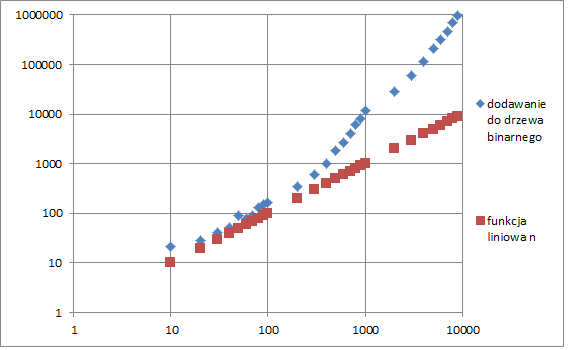
\includegraphics[scale=0.9]{1.png}
	\caption{Dodawanie do drzewa binarnego.}
	\label{fig:1}
	\end{figure}
	\begin{figure}
	\centering
	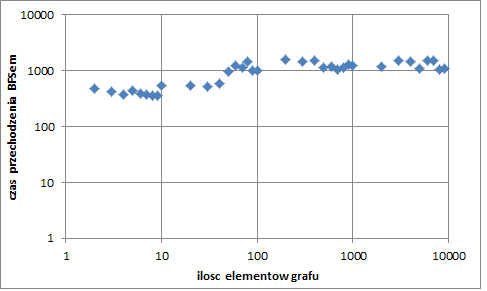
\includegraphics[scale=0.90]{2.png}
	\caption{Prszeszukiwanie drzewa binarnego.}
	\label{fig:2}
	\end{figure}

	\section{Komentarz}\label{sec:Komentarz}
	Do utworzenia dokumentacji wykorzystano system Doxygen. Funkcja pomiaru czasu dla systemu Windows pobrana ze strony dr. J. Mierzwy. Program skompilowano w środowisku Code::Blocks. Do stworzenia wykresu posłużono się pakietem MS Excel, sprawozdanie napisano używając systemu \LaTeX.
	
\begin{thebibliography}{99}
	\bibitem{1} http://pl.wikipedia.org/wiki/Przeszukiwanie\_w\_glab
	\bibitem{2} http://pl.wikipedia.org/wiki/Przeszukiwanie\_wszerz
\end{thebibliography}

\end{document}
